\documentclass{standalone}
\usepackage[T1]{fontenc}
\usepackage[latin2]{inputenc}
\usepackage[english]{babel}
\usepackage{tikz}
\usepackage{times}


% Packages needed to draw 
\usetikzlibrary{calc,through,backgrounds,positioning,fit}
\usetikzlibrary{shapes,arrows,shadows}
\usetikzlibrary{mindmap}
 
\begin{document}
 
% Defining different types of nodes %%%%%%%%%%%%%%%%%%%%%%%%%%%%%%%%%
\tikzstyle{place}=[shape=circle, draw, minimum height=10mm]
\tikzstyle{trig}=[shape=circle, draw, dashed, minimum height=10mm]
\tikzstyle{trans}=[shape=rectangle, draw, minimum height=6mm, minimum width=12mm]
 

% Inserting mindmap %%%%%%%%%%%%%%%%%%%%%%%%%%%%%%%%%%%%%%%%%%%%%%%%%%%
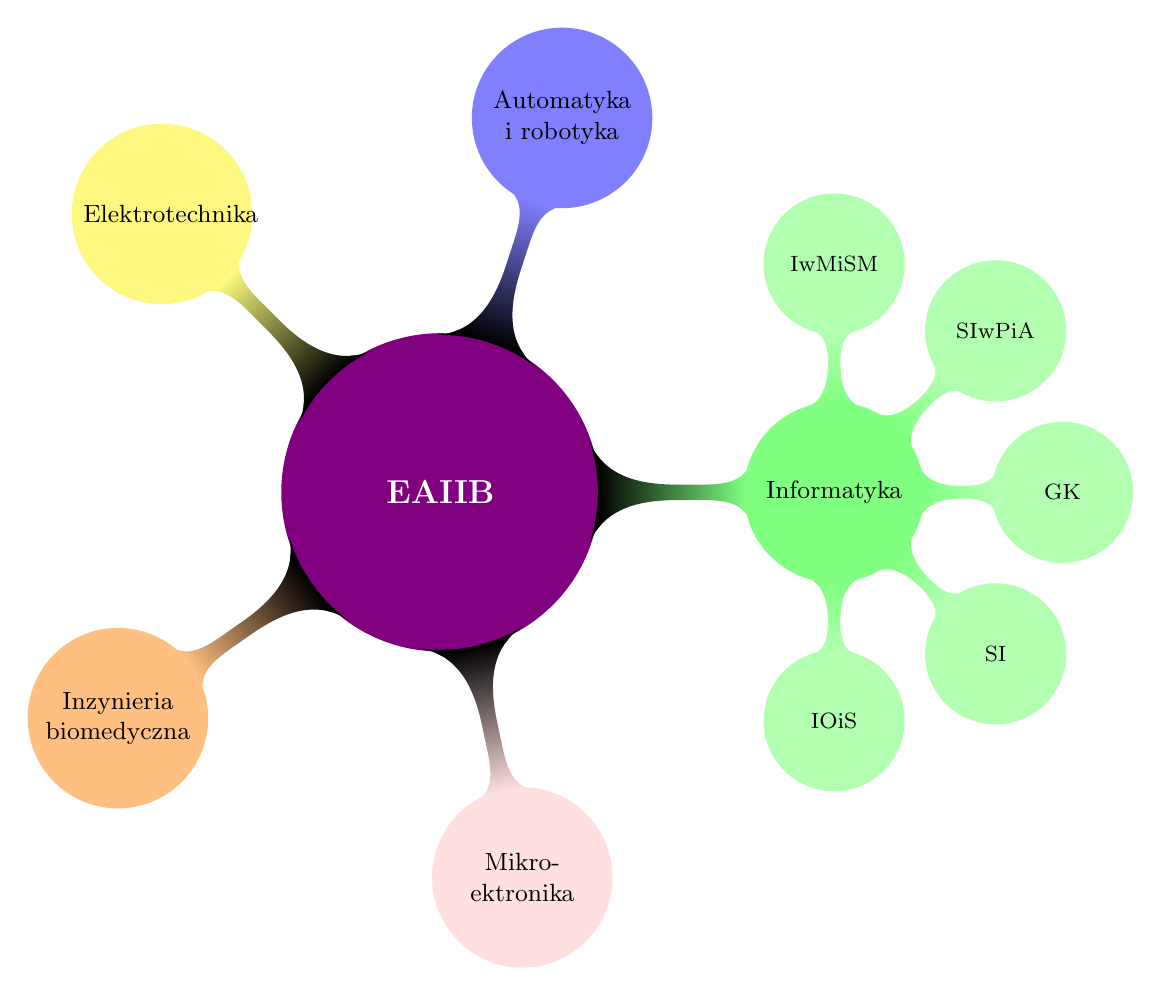
\begin{tikzpicture}[mindmap]

% Main node %%%%%%%%%%%%%%%%%%%%%%%%%%%%%%%%%%%%%%%%%%%%%%%%%%%%%%%%%%%
%\node [concept,concept color=red!50!blue, text=white] {\bf EAIiIB}
	%child[grow=90, concept color=green!30] {node[concept] {IOiS}}    
    %child[grow=90, concept color=green!30] {node[concept] {SIwPiA}}     
    %child[grow=90, concept color=green!30] {node[concept] {GK}}    
    %child[grow=90, concept color=green!30] {node[concept] {SI}}    
  %	child[grow=0, concept color=green!50] {node[concept] {Informatyka}
 %   child[grow=90, concept color=green!30] {node[concept] {IwMiSM}}
   % }   
  %	child[grow=72, concept color=blue!50] {node[concept] {Automatyka i 			robotyka}};
  % ...

\node [concept,concept color=red!50!blue, text=white] {\bf EAIIB}
  child[grow=0, concept color=green!50] {node[concept] {Informatyka}
  	child[grow=90, concept color=green!30] {node[concept] {IwMiSM}}
    child[grow=-90, concept color=green!30] {node[concept] {IOiS}}
    child[grow=45, concept color=green!30] {node[concept] {SIwPiA}}
    child[grow=0, concept color=green!30] {node[concept] {GK}}
    child[grow=-45, concept color=green!30] {node[concept] {SI}}
    %...  
  }
  child[grow=72, concept color=blue!50] {node[concept] {Automatyka i robotyka}}
  child[grow=135, concept color=yellow!50] {node[concept] {Elektrotechnika}}
  child[grow=215, concept color=orange!50] {node[concept] {Inzynieria biomedyczna}}
  child[grow=282, concept color=pink!50] {node[concept] {Mikro- \\ ektronika}}
  ;
  % ...

\end{tikzpicture}
 
\end{document}